\documentclass[12pt, a4paper]{report}
\linespread{1.3}
\setlength{\parindent}{1.25cm}

\usepackage[top=3cm,left=3cm,right=2cm,bottom=2cm]{geometry}
\usepackage{indentfirst}
\usepackage{amsmath, amsthm, amsfonts, amssymb}

\usepackage{graphicx}
\usepackage{color}
\usepackage{multicol}
\usepackage[normalem]{ulem}
\usepackage{wrapfig}
\usepackage{caption}
\usepackage{fancybox}
\usepackage[pdfstartview=FitH]{hyperref}
\usepackage{subfigure}

\usepackage[T1]{fontenc}		% Selecao de codigos de fonte.
\usepackage[utf8]{inputenc}
\usepackage[brazil]{babel}

\usepackage{array}
\usepackage{longtable}
\usepackage{pdfpages}

\usepackage{verbatim}
\usepackage{enumitem}   
\usepackage{natbib} % criação de linhas

%Includes "References" in the table of contents
\usepackage[nottoc]{tocbibind}

\graphicspath{{Figuras/}} % caminho padrao imagens
% ------ Remove nome capitulo da tag chapter ---------
\makeatletter
\def\@makechapterhead#1{%
  \vspace*{0\p@}%
  {\parindent \z@ \raggedright \normalfont
    \interlinepenalty\@M
    \Huge\bfseries  \thechapter.\quad #1\par\nobreak
    \vskip 30\p@
  }}
\makeatother
\begin{document}

%---------- CAPA -------------

\begin{figure}[ht]
\centering

\includegraphics[scale=0.15]{UFBA.jpg}
\end{figure}

\begin{center}
\sc{\large{Universidade Federal da Bahia - UFBA}} \\
\sc{\large{Instituto de Matemática - IM}} \\
\sc{\large{Departamento de Ciência da Computação - DCC}} \\
\sc{\small{Bacharelado em Sistemas de Informação - BSI}} \\
\sc{\small{Trabalho de Conclusão de Curso}} \\

\vspace{4cm}

\sc{\Large{Sistema Colaborativo de \\Avaliação
Docente - UFBA}}

\vspace{4.5cm}

\sc{\Large{Kênia Arruda Guimarães}}

\vspace{5.5cm}

\textbf{Salvador - Bahia} \\
Dezembro de 2019

\end{center}
\thispagestyle{empty}

%---------- FOLHA DE ROSTO -------------
\newpage
\begin{center}
\sc{\Large{Sistema Colaborativo de \\Avaliação
Docente - UFBA}

\vspace{4cm}

\large{Kênia Arruda Guimarães}
\end{center}

\vspace{4cm}

\begin{flushright}
\begin{minipage}{8.6cm}
Monografia apresentada como trabalho de conclusão de curso para o curso de Bacharelado em Sistemas de Informação do Departamento de Ciência da Computação na Universidade Federal da Bahia.

\vspace{0.5cm}
\textbf{Orientador}: Prof. Dr. Rodrigo Rocha Gomes e Souza.

\end{minipage}
\end{flushright}
 
\vspace{7cm}

\begin{center}
\textbf{Salvador - Bahia} \\
Dezembro de 2019
\end{center}


\presentationpage

%%%%%%%%%%%%%%%%%%%%%%
% Ficha Catalográfica
\newpage
\thispagestyle{empty}
\null\vfill
                  
\begin{center}
 Ficha catalográfica.
\begin{tabular}{|p{13.5cm}|}%{p{12cm}}
\hline
\begin{small}
\begin{verbatim}
Guimarães, Kênia Arruda
Sistema Colaborativo de Avaliação Docente - UFBA. / Kênia
Arruda Guimarães. - Salvador, 01, 2019.
60.:il.
Orientador: Rodrigo Rocha Gomes e Souza.
Monografia (Graduação) - UNIVERSIDADE FEDERAL DA BAHIA,
INSTITUTO DE MATEMÁTICA, 07 de dezembro de 2019.
TÓPICOS PARA FICHA CATALOGRÁFICA.
I.  Souza, Rodrigo Rocha Gomes e. 
II. UNIVERSIDADE FEDERAL DA BAHIA. INSTITUTO DE MATEMÁTICA.
III Título.
                                                  NUMERO CDD
\end{verbatim}
\end{small}
\\ \hline
\end{tabular}
\end{center}
\setcounter{page}{2} %truque para não numerar a página


%---------- BANCA EXAMINADORA -------------
\newpage
\begin{center}
\sc{\Large{Sistema Colaborativo de \\Avaliação Docente - UFBA}}

\vspace{2.2cm}

\large{Kênia Arruda Guimarães}
\end{center}

\vspace{2.2cm}

\begin{flushright}
\begin{minipage}{8.6cm} 
Monografia apresentada como trabalho de conclusão de curso para o curso de Bacharelado em Sistemas de Informação do Departamento de Ciência da Computação na Universidade Federal da Bahia.
\end{minipage}
\end{flushright}
 
\vspace{1cm}
\begin{center}
\Large \textbf{Banca Examinadora:}
\end{center}
\vspace{1.5cm}

\begin{flushright}
\begin{minipage}[l]{12cm}
\begin{center}
\uline{\hspace{10.5cm}} \\
Prof. Dr. Rodrigo Rocha Gomes e Souza (Orientador) \\ Universidade Federal da Bahia \\
\vspace{1cm}
\uline{\hspace{10.5cm}} \\

\vspace{1cm}
\uline{\hspace{10.5cm}} \\


\end{center}
\end{minipage}
\end{flushright}

%-----------Dedicatória----------------
\newpage
\vspace*{21cm}
\begin{flushright}
\textit{Dedico este trabalho à minha família}
\end{flushright}


%------------Agradecimentos------------
\newpage
\chapter*{Agradecimentos}
\thispagestyle{empty}
\par Aos meus pais que sempre estiveram ao meu lado me apoiando em cada decisão tomada. À minha noiva Juliana Alves Pereira que vem sendo meu maior suporte neste ciclo de aprendizado. À minha amiga Lina Mendes que me deu grande auxílio no design da aplicação. Aos meus amigos e em especial a Carlos Henrique e Ludmila Cruz que sempre tiveram muita paciência ao ouvir os desabafos quando ainda não tinha encontrado a solução para alguns dos obstáculos que encontrei durante a a execução deste projeto. E por fim, ao meu orientador Rodrigo Rocha Gomes e Souza pela excelente orientação, paciência e atenção prestados no desenvolvimento deste trabalho e a Universidade Federal da Bahia (UFBA) pelo espaço público de ensino que mesmo com todas as dificuldades encontradas forma profissionais excelentes que trarão conhecimento contribuindo para o desenvolvimento do nosso país.  

%------------Citação-------------------
\newpage
\vspace*{20cm}
\begin{flushright}
\begin{minipage}{7cm}
\begin{flushright}
\textit{
"Toda a ciência é nada mais do que um refinamento do pensamento cotidiano". \\
Albert Einstein}
\end{flushright}
\end{minipage}
\end{flushright}


%--------------Resumo-------------------
\newpage
\chapter*{Resumo}
\thispagestyle{empty}


%-------------Abstract------------------
\newpage
\chapter*{Abstract}
\thispagestyle{empty}

%-------------Índice--------------------
\newpage
\tableofcontents
\thispagestyle{empty}

% ----------- Lista de figuras ----------

\pdfbookmark[0]{\listfigurename}{lof}
\listoffigures
\cleardoublepage

%--------- Lista de tabelas ---------

\pdfbookmark[0]{\listtablename}{lot}
\listoftables
\cleardoublepage

%-------------Capítulo 1-----------------
\chapter{Introdução}

%-------------Capítulo 2-----------------
\chapter {Trabalhos Relacionados}

%-------------Capítulo 3-----------------
\chapter{Solução Proposta: SICAD}
\par Como solução para a problemática apresentada neste trabalho, está sendo proposto o Sistema Colaborativo de Avaliação Docente, SICAD, como ferramenta auxiliar para os discentes da Universidade Federal da Bahia utilizarem, a fim de disponibilizar feedbacks e avaliações sobre as disciplinas cursadas. 
\par O processo de concepção do SICAD foi realizado inicialmente como uma junção do trabalho já realizado pelo Sistema de Avaliação Docente, o SIAV\footnote{SIAV. Disponível em <\url{www.siav.ufba.br/siav/privado/index.faces}>. Acesso em: 11 nov. 2019.} disponibilizado pela UFBA\footnote{UFBA. Disponível em <\url{www.ufba.br}> . Acesso em: 1 nov. 2019.} com uma funcionalidade de se realizar comentários, que será especificada no subtópico a seguir. A partir deste escopo foram traçados os requisitos da solução que serão descritos abaixo.

\section{ Modelo Conceitual}
\par 
Por definição \textbf{modelo conceitual} é um conjunto de suposições baseadas no mundo real que indicarão as regas de negócio de um sistema \cite{mapaconceitual}.
\par A importância do desenvolvimento de um mapa conceitual no contexto deste trabalho é a representação gráfica do modelo proposto, referente os processos relacionados ao SICAD, a fim de que ele possa ser entendido de forma fluída.
\par Existem três macros processos   

\section{ Autenticação}
\par Inicialmente foi pensado em um login básico para autenticação no sistema, possuindo apenas um usuário e senha. Entende-se como login o processo para acessar um sistema informático restrito, utilizando credenciais que são previamente cadastradas pelo usuário nesse sistema com a finalidade da identificação do utilizador. Contudo, analisando o contexto o login abrangeria qualquer usuário logado na internet que possuísse o caminho do sistema, não sendo interessante pois os mesmos teriam acesso a resultados que possuem informações sensíveis.
\par Para delimitar o acesso ao SICAD, foi utilizado o módulo de \href{https://www.autenticacao.ufba.br}{autenticação} disponibilizado pela UFBA. Seu emprego segue o seguinte processo: a aplicação no ato do login, faz uma requisição à autenticação da UFBA e a mesma retorna o username \footnote{Username. Disponível em <\url{www.cartilha.cert.br/senhas/}> . Acesso em: 1 nov. 2019.} caso o usuário possua cadastro na universidade. Segue abaixo o fluxograma do processo.
\begin{figure}[!ht]
\centering
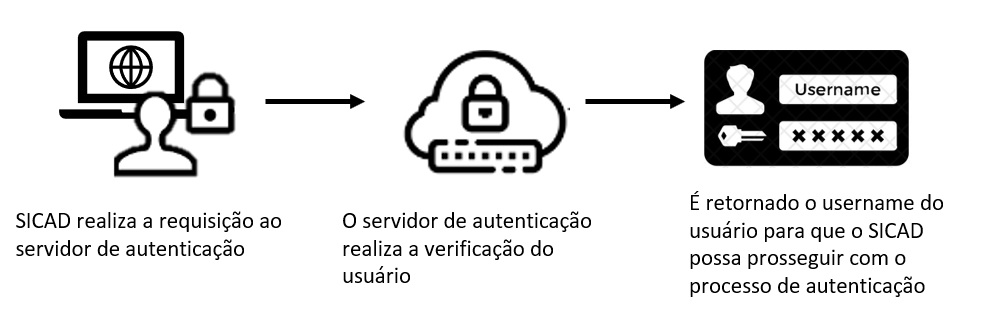
\includegraphics[scale=0.50]{processo_autenticacao.jpg}
\caption{Fluxograma da Requisição de Autenticação}
\label{fig:processo_autenticacao}
\end{figure}

\par Dessa forma o acesso ao SICAD é restrito a quem possuí cadastro na universidade, não expondo assim informações indevidas à usuários que não são elegíveis para utilizar o sistema.

\subsection{Usuário e Segurança}
\par No processo de desenvolvimento da autenticação ficou claro a necessidade da implementação de uma camada de segurança, visto que a resposta à requisição feita juntamente a UFBA retorna o username do usuário sem nenhum tipo proteção.
\par A segurança da informação é essencial no sentido de preservar o valor dessa informação que é chave para a maioria das funcionalidades do SICAD. Focando neste ponto foram implementadas rotinas para prover segurança nos processos executados pelo sistema que serão descritos nos passos abaixo:

\begin{itemize}
\item o usuário tenta logar no sistema, consequentemente disparando uma requisição para a autenticação da UFBA;
\item A UFBA executa todas as rotinas de validação.
Caso se obtenha uma resposta positiva, retorna o username do usuário sem proteção para a aplicação que solicitou a requisição;
\item O SICAD antes de persistir a informação no banco de dados, utiliza da tecnologia de criptografia Hash SHA256\footnote{Hash SHA256. Disponível em <\url{www.tsapps.nist.gov/publication/get_pdf.cfm?pub_id=910977}> . Acesso em: 2 nov. 2019.}, que será abordada no tópico 3.6. para criptografar o username que será chave para utilização do sistema. 
\end{itemize}
\par Para melhor fixação segue o fluxo do processo.
\begin{figure}[ht]
\centering
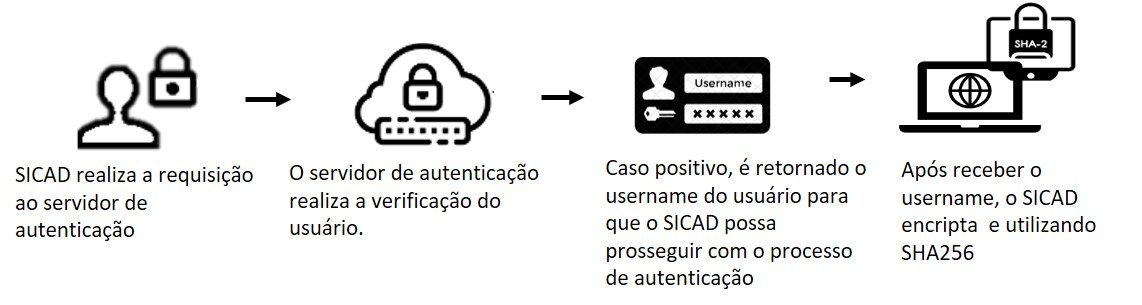
\includegraphics[scale=0.80]{fluxograma_criptografia.jpg}
\caption{Fluxograma do Processo de Criptografia}
\label{fig:processo_autenticacao}
\end{figure}
\par Por conseguinte, com o usuário criptografado e devidamente protegido, a integridade da informação será mantida sendo assim confiável que o usuário utilize o sistema de forma segura.

\section{ Perfis}
\par
A utilização de perfis de usuários está atrelada a restringir acesso à certas funcionalidades do sistema, que embora não elimine todos os riscos à segurança da informação mas diminui incidentes que possam ocorrer, comprometendo ao conjunto de critérios de segurança conhecido como o tripé da segurança da informação: \textbf{confidencialidade}, \textbf{integridade} e \textbf{disponibilidade}:
\begin{itemize}
\item \textbf{Confidencialidade:}é a garantia de que a informação é acessível somente por pessoas autorizadas a terem acesso; \cite{iso}
\item \textbf{Integridade:} é a garantia da exatidão e completeza  da  informação  e dos métodos de processamento; \cite{iso}
\item \textbf{Disponibilidade:} é a  garantia de que os usuários autorizados obtenham acesso à informação e aos ativos correspondentes sempre  que necessário. \cite{iso}
\end{itemize}
\par No SICAD foi implementado controle de perfis considerando critérios de segurança acima para que não ocorra a quebra dos mesmos gerando venerabilidades.
\subsection{O controle de Acesso}
\par Um processo de segurança essencial assegurado pelos critérios de segurança é o controle de acessos. É bastante difícil imaginar como qualquer sistema teria condições minímas de continuar funcionando sem ele e por isso é imprescindível sua implementação.
\subsection{Controle  de  Acesso  Baseado  em  Papéis }
\par Considerando o cenário dos acessos que foram pensados para o SICAD, foi escolhido o  modelo  de   \textbf{controle  de  acesso  baseado  em  papéis} devido ao seu adequamento à aplicação.
\par O modelo Role Based Access Control – RBAC flexibiliza o gerenciamento do controle de acesso através da adição de um componente que intermedeia usuários e permissões\cite{sandhu1997}. Considera quatro componentes básicos:
\begin{itemize}
\item \textbf{Usuários}: podem ser seres humanos ou outros agentes autônomos,tais como robôs,agentes de softwares e computadores;
\item \textbf{Permissões}: são os direitos de executar uma ou mais ações ou operações sobre objetos do sistema;
\item \textbf{Papéis}: são os intermediários entre os usuários e as permissões. Em vez de conceder permissões diretamente aos usuários, as permissões são concedidas aos papéis. Papéis são funções distintas dentro do sistema, como por exemplo Administrador, Moderador e etc. Usuários são associados a um ou mais papéis.  
\item \textbf{Sessões}: quando um usuário acessa o sistema, ele inicia uma \textbf{sessão}, durante  essa  sessão, pode haver  um  ou  mais  papéis ativos.Conforme a especificação do modelo, o usuário pode ter ou não o poder de decidir quais papéis ativar em um dado momento.
\end{itemize}
\par Partindo desses quatro componentes foram criados os papéis e permissões do sistema que poderá ser visualizado através da tabela abaixo:

% ######## init table ########
\begin{table}[h]
 \centering
% distancia entre a linha e o texto
 {\renewcommand\arraystretch{1.25}
 \begin{tabular}{ l l }
  \cline{1-1}\cline{2-2}  
    \multicolumn{1}{|p{3.850cm}|}{\textbf{Papel} \centering } &
    \multicolumn{1}{p{4.217cm}|}{\textbf{Permissão} \centering }
  \\  
  \cline{1-1}\cline{2-2}  
    \multicolumn{1}{|p{3.850cm}|}{Administrador} &
    \multicolumn{1}{p{4.217cm}|}{inclusão, alteração, visualização, bloqueio, desbloqueio de todos os módulos do sistema.}
  \\  
  \cline{1-1}\cline{2-2}  
    \multicolumn{1}{|p{3.850cm}|}{Utilizador} &
    \multicolumn{1}{p{4.217cm}|}{inclusão, visualização, bloqueio e desbloqueio nos módulos de comentários e avaliação.}
  \\  
  \hline
 \end{tabular} }
 \caption{Papéis e Permissões}
\end{table}
\par Um usuário poderá ser ter o papel de administrador ou utilizador. Como padrão quando o mesmo realiza o login já é atribuído à ele o papel de utilizador.
\par Além dos papéis e permissões, o SICAD conta com módulos que estão por sua vez associados aos papéis como é demonstrado pela tabela abaixo:
% ######## init table ########
\begin{table}[h]
 \centering
% distancia entre a linha e o texto
 {\renewcommand\arraystretch{1.25}
 
 \begin{tabular}{ l l }
  \cline{1-1}\cline{2-2}  
    \multicolumn{1}{|p{3.850cm}|}{\textbf{Módulo} \centering } &
    \multicolumn{1}{p{7.217cm}|}{\textbf{Papel} \centering }
  \\  
  \cline{1-1}\cline{2-2}  
    \multicolumn{1}{|p{3.850cm}|}{Comentário} &
    \multicolumn{1}{p{7.217cm}|}{Administrador, Utilizador}
  \\  
  \cline{1-1}\cline{2-2}  
    \multicolumn{1}{|p{3.850cm}|}{Avaliação} &
    \multicolumn{1}{p{7.217cm}|}{Administrador, Utilizador}
  \\  
    \cline{1-1}\cline{2-2}  
    \multicolumn{1}{|p{3.850cm}|}{Resultados} &
    \multicolumn{1}{p{7.217cm}|}{Administrador, Utilizador}
  \\  
    \cline{1-1}\cline{2-2}  
    \multicolumn{1}{|p{3.850cm}|}{Ajuda} &
    \multicolumn{1}{p{7.217cm}|}{Administrador, Utilizador}
  \\  
    \cline{1-1}\cline{2-2}  
    \multicolumn{1}{|p{3.850cm}|}{Carga} &
    \multicolumn{1}{p{7.217cm}|}{Administrador}
  \\  
    \cline{1-1}\cline{2-2}  
    \multicolumn{1}{|p{3.850cm}|}{Moderação} &
    \multicolumn{1}{p{7.217cm}|}{Administrador}
  \\  
    \cline{1-1}\cline{2-2}  
    \multicolumn{1}{|p{3.850cm}|}{Configurações} &
    \multicolumn{1}{p{7.217cm}|}{Administrador}
  \\  
  \hline
 \end{tabular} }
 \caption{Papéis e Módulos }
\end{table}
%rever https://www.teses.usp.br/teses/disponiveis/3/3141/tde-08032013-120904/publico/TeseEduardoTakeoUeda.pdf%
\par O  modelo  RBAC  permite  que  sejam  impostas  restrições na  ativação  de  papéis,de  modo  a  impedir  a  ativação  de papéis  com  conflitos  de  interesse  ou  mesmo  que um usuário possua papéis conflitantes.
\section{ Moderação}
\section{ Anonimato}
\section{ Segurança}
\section{ Principais Funcionalidades}

%-------------Capítulo 4-----------------
\chapter{Considerações Finais}

%-------------Bibliografia------------------

\renewcommand\bibname{Referências}
\bibliographystyle{apa}
\bibliographystyle{unsrt}
\bibliography{referencias}
\nocite{*}


%-------------Apêndice------------------
\appendix

\end{document}
